\documentclass[a4paper, 11pt]{article}
\usepackage[utf8]{inputenc}
\usepackage[swedish]{babel}
\usepackage{amsmath}
\usepackage{amssymb}
\usepackage{hyperref}
\usepackage{physics}
\usepackage{pgfplots}
\usepackage[margin=0.5in]{geometry}

\pgfplotsset{
	compat = 1.5.1,
	width = 1.2\linewidth,
	height = 1.2\linewidth
}

\newcommand{\N}{\mathbb{N}}
\newcommand{\Z}{\mathbb{Z}}
\newcommand{\Q}{\mathbb{Q}}
\newcommand{\R}{\mathbb{R}}
\newcommand{\C}{\mathbb{C}}
\newcommand{\proof}{\subparagraph{Bevis}}
\newcommand{\limit}[2]{\lim\limits_{#1\to #2}}
\newcommand{\Ordo}[1]{\mathcal{O}\left(#1\right)}
\newcommand{\deval}[4][]{\dv[#1]{#2}{#3} (#4)}
\newcommand{\integ}[4]{\int\limits_{#1}^{#2}#3\dd{#4}}

\title{Samanfatning av SF1673 Analys i en variabel}
\author{Yashar Honarmandi}
\date{\today}

\begin{document}\sloppy

\maketitle

\begin{abstract}
	Detta ær en sammanfattning av kursen SH1014 Modern fysik.
\end{abstract}

\pagenumbering{roman}
\thispagestyle{empty}

\newpage

\tableofcontents

\newpage

\pagenumbering{arabic}

\section{Mängder}

\paragraph{Delmängder}

Låt $A$ och $B$ vara mängder. $A$ är en delmängd av $B$ om det för varje $x \in A$ gäller att $x \in B$. Notation: $A \subset B$.

\section{Talföljder}

\subsection{Definitioner}

\paragraph{Definitionen av en talföjld}
En talföljd är en följd av tal $a_1, a_2, ...$ och betecknas $\left(a_n\right)_{n = 1}^\infty$.

\paragraph{Växande och avtagande talföljder}
En talföljd är växande om $a_{n + 1} \geq a_n$ för varje $n \geq 1$. Avtagande talföljder definieras analogt.

\paragraph{Uppåt och nedåt begränsade talföljder}
En talföljd är uppåt begränsad om det finns ett $M$ så att $a_n \leq M$ för alla $n \geq 1$.

\paragraph{Begränsade talföljder}
En talföljd är begränsad om den är både uppåt och nedåt begränsad.

\paragraph{Konvergens av talföljder}
En talföljd konvergerar mot ett gränsvärde $A$ om det för alla $\varepsilon > 0$ finns ett $N$ sådant att $\abs{a_n - A} < \varepsilon$ för varje $n > N$. Detta beteendet betecknas
\begin{align*}
	\lim_{n\to\infty} a_n = A.
\end{align*}

\paragraph{Divergenta talföljder}
En divergent talföljd är inte konvergent.

\paragraph{•}

\subsection{Satser}

\paragraph{Gränsvärden för kombinationer av talföljder}
Låt $\left(a_n\right)_{n = 1}^\infty, \left(b_n\right)_{n = 1}^\infty$ vara talföljder med gränsvärden $A$ och $B$. Då följer att
\begin{enumerate}
	\item[a)] $\left(a_n + b_n\right)_{n = 1}^\infty$ är konvergent med gränsvärdet $A + B$.
	\item[b)] $\left(a_n b_n\right)_{n = 1}^\infty$ är konvergent med gränsvärdet $AB$.
	\item[c)] om $B \neq 0$ är $\left(\frac{a_n}{b_n}\right)_{n = 1}^\infty$ konvergent med gränsvärdet $\frac{A}{B}$.
	\item[d)] om $a_n \leq b_n$ för varje $n$ så gäller att $A \leq B$.
\end{enumerate}

\subparagraph{Bevis}
Aa.

\paragraph{Växande och uppåt begränsade talföljder}
Om $\left(a_n\right)_{n = 1}^\infty$ är en växande och uppåt begränsad talföljd så är den konvergent och
\begin{align*}
	\lim_{n\to\infty} a_n = \sup{\{a_n: n \geq 1\}}
\end{align*}
Det analoga gäller för avtagande och nedåt begränsade mängder.

\subparagraph{Bevis}
Oo.

\paragraph{Gränsvärde för potenser}
\begin{align*}
	\lim_{n\to\infty} n^p =
	\begin{cases}
		\infty, & p > 0\\
		0,      & p < 0
	\end{cases}
\end{align*}

\section{Funktioner}

\subsection{Definitioner}

\paragraph{Definition av en funktion}

Låt $X, Y$ vara mängder. En funktion $f: X\to Y$ är ett sätt att till varje element $x \in X$ tilldela ett välbestämt element $y\in Y$. Vi säger att $x$ avbildas på $y$ och att $y$ är bilden av $x$. $x$ kallas argumentet till $f$. $X$ kallas funktionens definitionsmängd, och betecknas även $D_f$. $Y$ kallas funktionen målmängd.

\paragraph{Värdemängd}

Värdemängden till $f: X\rightarrow Y$ definieras som:
\begin{align}
	V_f=\left \{y\in Y: y=f(x)\textnormal{ för något }x\in X\right \}\nonumber
\end{align}
alltså alla värden $f$ antar.

\paragraph{Injektivitet}

$f$ är injektiv om det för varje $x_1, x_2 \in X$ gäller att om $f(x_1)=f(x_2)$ så är $x_1=x_2$.

\paragraph{Surjektivitet}

$f$ är surjektiv om $V_f=Y$.

\paragraph{Bijektivitet}

Om $f$ är injektiv och surjektiv, är $f$ bijektiv.

\paragraph{Inversa funktioner}

Låt $f: X \to Y$ vara en bijektiv funktion. Inversen till $f$ är avbildningen $f^{-1}: Y\to X$ som ges av $f^{-1}(y)=x$, där $y=f(x)$. Funktioner som har en invers kallas inverterbara.

\paragraph{Växande och avtagande funktioner}

En funktion $f$ är växande på en mängd $M\in D_f$ om det för varje $x,y\in M: x<y$ gäller att $f(x)\leq f(y)$. Om $M=D_f$ kallas $f$ växande. Avtagande funktioner definieras analogt.

\paragraph{Strängt växande och avtagande funktioner}

En funktion $f$ är strängt växande på en mängd $M\in D_f$ om det för varje $x,y\in M: x<y$ gäller att $f(x)<f(y)$. Om $M=D_f$ kallas $f$ strängt växande. Strängt avtagande funktioner definieras analogt.

\paragraph{Monotona funktioner}

Om en funktioner är antingen strängt växande respektiva strängt avtagande eller växande respektiva avtagande i ett intervall, är den strängt monoton respektiva monoton.

\paragraph{Uppåt och nedåt begränsade funktioner}

En funktion $f$ är uppåt begränsad om $V_f$ är uppåt begränsad. Nedåt begränsade funktioner definieras analogt. Om funktioner saknar övre eller nedra begrensning är den uppåt eller nedåt obegränsad.

\paragraph{Trigonometriska funktioner}

Betrakta enhetssirkeln i figur \ref{fig:unit_circle}, med radie $1$.

\begin{figure}[!ht]
	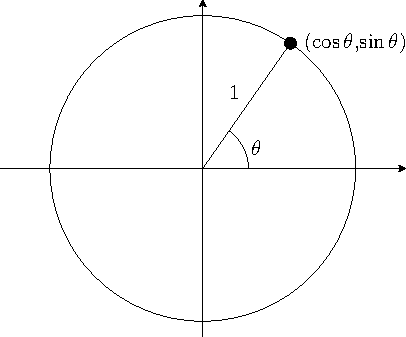
\includegraphics[width=\linewidth]{./Images/unit_circle/unit_circle.pdf}
	\caption{Enhetssirkeln.}
	\label{fig:unit_circle}
\end{figure}

Man tenker sig en punkt på cirkeln enligt figuren, var linjen från cirkelns centrum till cirkeln bildar en vinkel $\theta$ med $x$-axeln. Denna vinkeln startar när punkten på cirkeln ligger på den positiva sidan av $x$-axeln, och ökar moturs. Från denna konstruktionen definieras $\sin$ och $\cos$ utifrån $x$- och $y$-koordinaterna till punkten för en given $\theta$, var $\theta$ mäts i radianer. Vi definierar även $\tan\theta=\frac{\sin\theta}{\cos\theta}$.

Från definitonerna ser vi at $\sin x$ och $\cos x$ är definierade för alla $x\in\R$, medan $\tan x$ är definierad för alla $x\neq \frac{\pi}{2}n, n\in\Z$.

\paragraph{Radianer}

Radianer är ett mått på vinklar som är baserad på enhetscirkeln. Om man tenker sig att punkten i figur \ref{fig:unit_circle} beväger sig från startpunktet och till nån 

\paragraph{Trigonometriska funktioners egenskaper}

Från definitionen av dom trigonometriska funktionerna följer många egenskaper vid dissa. Några essensiella är listad under:

\begin{align*}
	&\cos^2x + \sin^2x = 1\\
	&\sin\left(\theta + 2\pi n\right) = \sin\theta\\
	&\cos\left(\theta + 2\pi n\right) = \cos\theta\\
	&\sin\left(\theta - \frac{\pi}{2}\right) = \cos\theta\\
	&\cos\left(\theta + \frac{\pi}{2}\right) = \sin\theta\\
	&\sin\left(-\theta\right) = -\sin\theta\\
	&\cos\left(-\theta\right) = -\cos\theta\\
	&\sin\left(\theta+\pi\right) = -\sin\theta\\
	&\cos\left(\theta+\pi\right) = -\cos\theta
\end{align*}

\paragraph{Inversa trigonometriska funktioner}

Låt $f:\left[-\frac{\pi}{2},\frac{\pi}{2}\right]\to [-1,1]$ sådan att $f(x)=\sin x$. Inversen till denna funktionen betecknas $f^{-1}(x)=\arcsin x$.

Låt $f:[0,\pi]\to [-1,1]$ sådan att $f(x)=\cos x$. Inversen till denna funktionen betecknas $f^{-1}(x)=\arccos x$.

Låt $f:(-\infty,\infty)\to \left(-\frac{\pi}{2},\frac{\pi}{2}\right)$ sådan att $f(x)=\tan x$. Inversen till denna funktionen betecknas $f^{-1}(x)=\arctan x$.

\paragraph{Exponentialfunktionen}

I häftet definieras inte exponentialfunktionen $a^x, a>1$, utan den antas vara en strängt växande funktion med värdemängd $(0,\infty)$ som uppfyller
\begin{align*}
	&a^0 = 1\\
	&a^1 = a\\
	&a^{x + y} = a^x a^y\\
	&a^{-x} = \frac{1}{a^x}\\
	&\left(a^x\right)^y = a^{xy}
\end{align*}

\paragraph{Logaritmfunktionen}

Låt $f:\mathbb{R}\to (0,\infty)$ sådan att $f(x) = a^x$ för något $a > 1$. Inversen till denna funktionen betecknas som $f^{-1}(x) = \log_a x$.

\paragraph{Absolutbelopp}

Absolutbeloppet definieras som $\abs{x} = \sqrt{x^2}$. Detta impliserar att
\begin{align*}
	\abs{x} =
	\begin{cases}
		-x, & x < 1\\
		x,  & x \geq 1
	\end{cases}
\end{align*}
 
\paragraph{Kontinuitet}
Låt $f$ vara en reellvärd funktion med $D_f\subset\R$, sådan att varje punkterad omgivning till $x = a$ innehåller punkter från $D_f$ och $a\in D_f$. $f$ är kontinuerlig i $a$ om
\begin{align*}
	\lim\limits_{x\to a}f(x) = f(a).
\end{align*}

\subsection{Satser}

\paragraph{Trigonometriska funktioner med vinkelsummor}
\begin{align*}
	\sin\left(x+y\right) = \sin x\cos y + \cos x\sin y\\
	\cos\left(x+y\right) = \cos x\cos y - \sin x\sin y
\end{align*}

\paragraph{Cosinussatsen}

Låt $a,b,c$ vara sidorna i en triangel och $\theta$ vinkeln där sidlängderna $a$ och $b$ möts. Då gäller att
\begin{align*}
	c^2=a^2+b^2-2ab\cos\theta
\end{align*}

\paragraph{Logaritmfunktionens egenskaper}

Låt $a > 1$. Då gäller att
\begin{align}
	&\log_a 1 = 0 \label{eq:log_1}\\
	&\log_a\left(xy\right) = \log_a\left(x\right) + \log_a\left(y\right) \label{eq:log_prod}\\
	&\log_a\left(x^y\right) = y\log_a\left(x\right) \label{eq:log_pow}
\end{align}

\subparagraph{Bevis}

Alla identiteter är baserade på inverterbarheten till exponentialfunktionen - $a^{\log_a x} = x$ - och injektiviteten till exponentialfunktionen, samt reglerna som exponentialfunktionen uppfyllar.

Ekvation \ref{eq:log_1} fås från att $a^{\log_a 1} = 1$ och att $a^0 = 1$. Eftersom exponentialfunktionen är injektiv, är det bevisad.

Ekvation \ref{eq:log_prod} fås från att $a^{\log_a xy} = xy$ och att $a^{\log_a x + \log_a y} = a^{\log_a x}a^{\log_a y}=xy$.

Ekvation \ref{eq:log_pow} fås från att $a^{\log_a x^y} = x^y$ och att $a^{y\log_a x} = \left(a^{\log_a x}\right)^y = x^y$.

\paragraph{Absolutbeloppens egenskaper}

\begin{align}
	&\abs{xy} = \abs{x}\abs{y} \label{eq:abs_prod} \\
	&\abs{x + y} \leq \abs{x} + \abs{y} \label{eq:abs_sum}
\end{align}

\subparagraph{Bevis}

Kommer kanskje någon gång.

\section{Gränsvärden}

\subsection{Definitioner}

\paragraph{Gränsvärde vid oändligheten}
Låt $f$ vara en funktion definierad i $(a, \infty)$. $f$ konvergerar mot gränsvärdet $A$ när $x\to\infty$ om det for varje $\varepsilon > 0$ finns ett $N$ sådant att $\abs{f(x) - A} < \varepsilon$ för varje $x > N$. Detta skrivs
\begin{align*}
	\lim_{x \to \infty} f(x) = A
\end{align*}
eller $f(x) \to A$ när $x \to \infty$.

\paragraph{Divergens}
Om det för en funktion $f$ inte finns ett sådant $A$, sägs $f$ vara divergent då $x \to \ infty$.

\paragraph{Det oegentliga gränsvärdet}
Låt $f$ vara en funktion definierad i $(a, \infty)$. $f$ har det oegentliga gränsvärdet $\infty$ då $x \ to \infty$ om det för varje $M$ finns ett $N$ sådant att $f(x) > M$ för varje $x > N$. Detta skrivs
\begin{align*}
	\lim_{x \to \infty} f(x) = \infty.
\end{align*}

\paragraph{Lokalt gränsvärde}
Låt $f$ vara en reellvärd funktion med $D_f\subset\R$ sådan att varje punkterad omgivning till $x = a$ innehåller punkter i $D_f$. $f$ konvergerar mot $A$ när $x$ går mot $a$ om det för varje $\varepsilon > 0$ finns ett $\delta > 0$ sådant att $\abs{f(x) - A} < \varepsilon$ för varje $x\in D_f$ som uppfyllar $0 < \abs{x - a} < \delta$. Detta skrivs $\lim\limits_{x\to a} f(x) = A$.

\paragraph{Vänster- och högergränsvärden}
Vid att endast studera $x > a$ eller $x < a$ kan man definiera ett vänster- och högergränsvärde för en funktion $f$. Dessa skrivs $\lim\limits_{x\to a^-} f(x) = A$ eller $\lim\limits_{x\to a^+} f(x) = A$. För en funktion $f$ definierad i en punkterad omgivning till $a$ existerar $\lim\limits_{x\to a} f(x)$ om och endast om vänster- och högergränsvärden existerar och är lika.

\paragraph{Det oegentliga lokala gränsvärdet}
Låt $f$ vara en funktion sådan att varje punkterad omgivning till  $x = a$ innehåller punkter i $D_f$. $f$ har det oegentliga gränsvärdet $\infty$ då $x\to a$ om det för varje $K$ finns ett $delta$ sådant att $f(x) > K$ för varje $x\in D_f$ som uppfyll	ar $0 < \abs{x - a} < \delta$

\subsection{Satser}

\paragraph{Gränsvärden för kombinationer av funktioner}
Låt $f,g$ vara kontinuerliga funktioner sådana att $f(x)\to A, g(x)\to B$ när $x\to\infty$. Då gäller att
\begin{itemize}
	\item[a)] $f(x) + g(x)\to A + B$ när $x\to\infty$.
	\item[b)] $f(x)g(x)\to AB$ när $x\to\infty$.
	\item[c)] om $B\neq 0$ så följer att $\frac{f(x)}{g(x)}\to\frac{A}{B}$ när $x\to\infty$.
	\item[d)] om $f(x)\leq g(x)$ för alla $x\in (a,\infty)$ så gäller att $A\leq B$.
\end{itemize}

\subparagraph{Bevis}
Mjo.

\paragraph{Gränsvärden och supremum}
Låt $f: (a, \infty)\to\R$ för något $a\in\R$ vara växande och uppåt begränsad. Då gäller att
\begin{align*}
	\lim\limits_{n\to\infty} = \sup{f(x): x\geq a}.
\end{align*}

\subparagraph{Bevis}
Nä.

\paragraph{Standardgränsvärden}
Låt $a > 1, b > 0$. Då gäller att
\begin{align*}
	\lim\limits_{x\to\infty}\frac{a^x}{x^b} = \infty \\
	\lim\limits_{x\to\infty}\frac{x^b}{\log_a x} = \infty
\end{align*}

\subparagraph{Bevis}
Orkar inte.

\section{Derivata}

\subsection{Definitioner}

\paragraph{Derivatans definition}
Låt $f$ vara en funktion definierad i en omgvning krin $x_0$. $f$ är deriverbar i $x_0$ om
\begin{align*}
	\eval{\dv{f}{x}}_{x_0} &= \dv{f}{x} (x_0) = f'(x_0) \\
	                           &= \lim\limits_{h\to 0}\frac{f(x_0 + h) - f(x_0)}{h}
\end{align*}
existerar. Värdet kallas derivatan i $x_0$.

\paragraph{Deriverbara funktioner}
Om en funktion $f$ är deriverbar i alla punkter i definitionsmängden, är funktionen deriverbar. Funktionen $f' = \dv{f}{x}$ med $D_{f'} = D_f$ kallas derivatan.

\paragraph{Minima och maxima}
En funktion $f$ har ett lokalt maximum i $x_0$ om det finns en omgivning $I$ till $x_0$ så att $f(x)\leq f(x_0)$ för alla $x\in I\cap D_f$. Det analoga gäller för ett lokalt minimum. Om $f$ har antingen ett lokalt maximum eller minimum i $x_0$ har $f$ ett lokalt extrempunkt i $f$.

\paragraph{Stationära punkt}
En funktion $f$ har ett stationärt punkt $x_0$ om $\dv{f}{x}\eval_{x_0} = 0$.

\paragraph{Inflexionspunkt}
Låt $f$ vara en funktion definierad på ett intervall $I$. En punkt $x_0\in I$ sägs vara en inflexionspunkt till $f$ om det finns ett $\delta > 0$ sådan att $f$ är konvex i $[x_0 - \delta, x_0]$ eller $[x_0, x_0 + \delta]$ och konkav i det andra.

\paragraph{Globala maxima och minima}
En funktion $f$ har ett globalt maximum i $x_0$ om $f(x)\leq f(x_0$ för varje $x\in D_f$.

\paragraph{Taylorpolynomet}
Låt $f$ vara $n$ gånger deriverbar. Polynomet
\begin{align*}
	p_n(x) = \sum\limits_{i = 0}{n}\frac{\dv[i]{f}{x} (0)}{i!}(x - a)^i
\end{align*}
kallas Taylorpolynomet av grad $n$ till $f$ kring $a$. Specialfallet där $a = 0$ kallas Maclaurinpolynomet till $f$ av grad $n$.

\subsection{Satser}

\paragraph{Derivata och kontinuitet}
Låt $f$ vara deriverbar i $(a, b)$. Då är $f$ kontinuerlig i $(a, b)$.

\proof
Kan man tänka.

\paragraph{Derivationsregler}
Låt $f, g$ vara deriverbara i punkten $x$. Då följer att $f + g, fg$ är deriverbara i $x$. Derivatorna har sambandet
\begin{align*}
	\eval{\dv{x}(f + g)}_x &= \left(\dv{f}{x} + \dv{g}{x}\right)\eval_x, \\
	\eval{\dv{x}(af)}_x    &= a\dv{f}{x}\eval_x, a\in\R, \\
	\eval{\dv{x}(fg)}_x    &= \left(f\dv{g}{x} + g\dv{f}{x}\right)\eval_x. \\
\end{align*}
Om $g(x)\neq 0$ är även $\frac{f}{g}$ deriverbar i $x$ och
\begin{align*}
	\dv{x}\frac{f}{g}\eval_x = \frac{\left(g\dv{f}{x} - f\dv{g}{x}\right)\eval_x}{g^2(x)}.
\end{align*}

\proof
Inte omöjligt.

\paragraph{Kedjeregeln}
Låt $f$ vara deriverbar i $y$, $g$ deriverbar i $x$ och $y = g(x)$. Då är den sammansatta funktionen $f\circ g$ deriverbar och
\begin{align*}
	\dv{x}(f\circ g)\eval_x = \dv{x}f\eval_{g(x)}\cdot\dv{x}g\eval_x.
\end{align*}

\proof

\paragraph{Derivatan av inversfunktioner}
Låt $f$ vara en deriverbar och inverterbar funktion. Då är inversen $f^{-1}$ deriverbar i alla punkter $y = \dv{x}f\eval_x$ där $\dv{x}f\eval_x\neq 0$ med derivatan
\begin{align*}
	\dv{y}f^{-1}\eval_y = \frac{1}{\dv{x}f\eval_x}.
\end{align*}

\proof

\paragraph{Extrempunkt och derivata}
Låt $f$ vara deriverbar i $x_0$ och ha en lokal extrempunkt i $x_0$. Då är $\dv{f}{x}\eval_{x_0} = 0$.

\proof

\paragraph{Rolles sats}
Låt $f$ vara kontinuerlig på $[a, b]$, deriverbar på $(a, b)$ så att $f(a) = f(b)$. Då existerar $p\in (a, b)$ så att $\dv{f}{x}\eval_p = 0$.

\proof

\paragraph{Generaliserade medelvärdessatsen}
Låt $f$ och $g$ vara reellvärda, kontinuerliga på $[a, b]$ och deriverbara på $(a, b)$. Då existerar $p\in (a, b)$ så att
\begin{align*}
	\dv{f}{x}\eval_p(g(b) - g(a)) = \dv{g}{x}\eval_p(f(b) - f(a)).
\end{align*}
Om $g(a)\neq g(b)$ och $\dv{g}{x}\eval_p\neq 0$, gäller
\begin{align*}
	\frac{\dv{f}{x}\eval_p}{\dv{g}{x}\eval_p} = \frac{f(b) - f(a)}{g(b) - g(a)}.
\end{align*}

\subparagraph{Medelvärdesatsen}
Välj $g(x) = x$. Detta ger
\begin{align*}
	\dv{f}{x}\eval_p(b - a) = f(b) - f(a).
\end{align*}

\proof
Använd Rolles sats.

\paragraph{Följder av dessa satser}
Låt $f$ vara deriverbar på $(a, b)$. Då gäller:
\begin{itemize}
	\item $\dv{f}{x}(x) = 0$ för varje $x\in (a, b)$ omm $f$ är konstant på $(a, b)$.
	\item $\dv{f}{x}(x)\geq 0$ för varje $x\in (a, b)$ omm $f$ är växande på $(a, b)$.
	\item $\dv{f}{x}(x) > 0$ implicerar att $f$ är strängt växande på $(a, b)$.
	\item $\dv{f}{x}(x)\leq 0$ för varje $x\in (a, b)$ omm $f$ är avtagande på $(a, b)$.
	\item $\dv{f}{x}(x) < 0$ implicerar att $f$ är strängt avtagande på $(a, b)$.
\end{itemize}

\proof

\paragraph{L'Hôpitals regel}
Låt $f, g$ vara reellvärda, deriverbara funktioner i en omgivning $I$ av $a$ sådana att
\begin{align*}
	\lim\limits_{x\to a}f(x) = \lim\limits_{x\to a}g(x) = 0.
\end{align*}
Då gäller att
\begin{align*}
	\lim\limits_{x\to a}\frac{f(x)}{g(x)} = \lim\limits_{x\to a}\frac{\dv{f}{x} (x)}{\dv{g}{x} (x)}.
\end{align*}

\proof

\paragraph{Oändliga kvoter}
Låt
\begin{align*}
	\lim\limits_{x\to a}\frac{\dv{f}{x} (x)}{\dv{g}{x} (x)} &= L, \\
	\limit{x}{a}f(x)                                        &= \pm\infty, \\
	\limit{x}{a}g(x)                                        &= \pm\infty.
\end{align*}
Då gäller att
\begin{align*}
	\limit{x}{a}\frac{f(x)}{g(x)} = L.
\end{align*}

\proof

\paragraph{Konvexitet och derivata}
Låt $f$ vara deriverbar i $(a, b)$. Då är $f$ konvex i $(a, b)$ omm $\dv{f}{x}$ är växande i $(a, b)$.

\proof

\paragraph{Andrederivata och konvexitet}
Låt $f$ vara två gånger deriverbar i $(a, b)$. Då är $\dv[2]{f}{x} (x)\geq 0$ för varje $x\in (a, b)$ omm $f$ är konvex.

\proof

\paragraph{Andrederivata och inflexionspunkt}
Låt $f$ vara två gånger deriverbar och låt $\dv[2]{f}{x}$ vara kontinuerlig. Om $f$ har en inflexionspunkt i $x_0$ så är $\dv[2]{f}{x} (x_0) = 0$.

\proof

\paragraph{Taylors formel}
Låt $f$ vara $n$ gånger deriverbar och definierad i en omgivning av $0$, sådan att $\dv[n]{f}{x}$ är kontinuerlig. Då är
\begin{align*}
	f(x) = \sum\limits_{i = 0}^{n - 1}\frac{\dv[i]{f}{x} (0)}{i!}x^i + \frac{\dv[n]{f}{x} (\alpha)}{n!}x^n
\end{align*}
för något $\alpha\in [0, x]$. Kring en godtycklig punkt $a$ blir formeln
\begin{align*}
	f(x) = \sum\limits_{i = 0}^{n - 1}\frac{\dv[i]{f}{x} (a)}{i!}(x - a)^i + \frac{\dv[n]{f}{x} (\alpha)}{n!}(x - a)^n
\end{align*}
för något $\alpha\in (a, x)$.

\proof

\paragraph{Taylors formel och stora ordo}
Låt $f$ vara $n$ gånger deriverbar och $\dv[n]{f}{x}$ vara kontinuerlig i en omgivning av $0$. Då är
\begin{align*}
	f(x) = \sum\limits_{i = 0}^{n - 1}\frac{\dv[i]{f}{x} (0)}{i!}x^i + \Ordo{x^n}.
\end{align*}

\proof

\section{Serier}

\subsection{Definitioner}

\paragraph{Delsummor}
Låt $\left(a_i\right)_{i = 1}^\infty$ vara en talföljd. Den motsvarande delsumman är
\begin{align*}
	s_n = \sum\limits_{i = 1}^{n}a_i.
\end{align*}

\paragraph{Serier}
En serie definieras som
\begin{align*}
	\sum\limits_{i = 1}^{\infty}a_i = \limit{n}{\infty}s_n.
\end{align*}

\paragraph{Konvergens}
Om $\limit{n}{\infty}s_n$ existerar, är serien konvergent mot dens summa. Annars är den divergent.

\paragraph{Geometriska serier}
En geometrisk serie är på formen $a_i = x^i$.

\paragraph{Absolut konvergens}
Serien $\sum\limits_{i = 1}^{\infty}a_i$ är absolutt konvergent om $\sum\limits_{i = 1}^{\infty}\abs{a_i}$ är konvergent.

\paragraph{Taylorserier}
Låt $f$ vara oändligt deriverbar. Funktionens Taylorserie kring $a$ är
\begin{align*}
	s = \sum\limits_{i = 1}^{\infty}\frac{\dv[i]{f}{x}(a)}{i!}(x - a)^i.
\end{align*}

\paragraph{Konvergensradie}
Enligt ekvation \ref{eq:taylor_formula} är
\begin{align*}
	f(x) - p_{n-1}(x) = R_n(x) = \frac{\dv[n]{f}{x} (\alpha)}{n!}(x - a)^n.
\end{align*}
$f$ konvergerar mot sin Taylorserie om denna resttermen går mot $0$ när $n\to\infty$ för ett givet $x$. Detta händer för $x$ så att $\abs{x -a} < r$, där $r$ är Taylorseriens konvergensradie.

\subsection{Satser}

\paragraph{Seriers egenskaper}
Låt $\sum\limits_{i = 1}^{\infty}a_i, \sum\limits_{i = 1}^{\infty}b_i$ vara två konvergenta serier. Då gäller
\begin{align*}
	&\sum\limits_{i = 1}^{\infty}(a_i + b_i) = \sum\limits_{i = 1}^{\infty}a_i + \sum\limits_{i = 1}^{\infty}b_i, \\
	&\sum\limits_{i = 1}^{\infty}ca_i = c\sum\limits_{i = 1}^{\infty}a_i, c\in\R.
\end{align*}

\proof

\paragraph{Konvergens och termernas beteende}
Om $\sum\limits_{i = 1}^{\infty}a_i$ är konvergent är $\limit{i}{\infty}a_i = 0$.

\proof
Låt $s_n$ beteckna seriens delsumma och $S$ dens summa. Vi har
\begin{align*}
	a_n = s_n - s_{n - 1}.
\end{align*}
Om serien är konvergent, kan vi räkna ut gränsvärdet enligt
\begin{align*}
	\limit{n}{\infty}a_n = \limit{n}{\infty}(s_n - s_{n - 1}) = S - S = 0.
\end{align*}

\paragraph{Summan av en geometrisk serie}
Om $\abs{x} < 1$ är
\begin{align*}
	\sum\limits_{i = 1}^{\infty}x^i = \frac{1}{1 - x}.
\end{align*}

\proof
Betrakta $s_n - xs_n = 1 - x^{n + 1}$. Detta ger
\begin{align*}
	\sum\limits_{i = 1}^{n}x^i = \frac{1 - x^{n + 1}}{1 - x}.
\end{align*}
Om $\abs{x} < 1$ har man
\begin{align*}
	\sum\limits_{i = 1}^{\infty}x^i = \frac{1}{1 - x}.
\end{align*}

\paragraph{Jamförelse av termer och konvergens}
Låt $0\leq a_i\leq b_i$ för alla $i$. Då gäller att
\begin{itemize}
	\item om $\sum\limits_{i = 1}^{\infty}b_i$ är konvergent är $\sum\limits_{i = 1}^{\infty}a_i$ konvergent.
	\item om $\sum\limits_{i = 1}^{\infty}a_i$ är divergent är $\sum\limits_{i = 1}^{\infty}b_i$ divergent.
\end{itemize}

\proof

\paragraph{Kvoten av termer och konvergens}
Låt $\sum\limits_{i = 1}^{\infty}a_i, \sum\limits_{i = 1}^{\infty}b_i$ vara två positiva serier vars termer uppfyller
\begin{align*}
	\limit{i}{\infty}\frac{a_i}{b_i} = K\neq 0.
\end{align*}
Då konvergerar $\sum\limits_{i = 1}^{\infty}a_i$ om och endast om $\sum\limits_{i = 1}^{\infty}b_i$ konvergerar.

\proof

\paragraph{Absolut konvergens och konvergens}
En absolut konvergent serie är konvergent.

\proof

\paragraph{Summan av potenser}
Serien
\begin{align*}
	\sum\limits_{i = 1}^{\infty}\frac{1}{i^p}
\end{align*}
är konvergent om och endast om $p > 1$.

\proof

\section{Integraler}

\subsection{Definitioner}

\paragraph{Trappfunktioner}
En trappfunktion på intervallet $[a, b]$ är på formen
\begin{align*}
	\Psi(x) =
	\begin{cases}
		c_1, a\leq x\leq x_1 \\
		c_2, x_1\leq x\leq x_2 \\
		\vdots \\
		c_n, x_{n - 1}\leq x\leq x_n \\
	\end{cases}
\end{align*}
Mängden av alla $x_i$ kallas en uppdelning av intervallet och intervallerna $[x_{i - 1}, x_i]$ kallas delintervall av uppdelningen.

\paragraph{Integralen av en trappfunktion}
Låt $\Psi$ vara en trappfunktion. Då definieras integralen av denna som
\begin{align*}
	\integ{a}{b}{\Psi(x)}{x} = \sum\limits_{i = 1}^{n}c_i{x_i - x_{i - 1}}.
\end{align*}

\paragraph{Övertrappor och undertrappor}
En övertrappa $\Psi$ för en funktion $f$ är en funktion så att
\begin{align*}
	f(x)\leq \Psi(x).
\end{align*}
Undertrappor definieras analogt. Integralerna av dessa kallas översummor och undersummor.

\paragraph{Integrerbarhet}
Låt $f$, definierad på $[a, b]$, vara en begränsad funktion, $L(f)$ vara mängden av alla undersummor till $f$ och $U(f)$ mängden av alla översummor till $f$. $L(f)$ är uppåt begränsad av talen i $U(f)$ och vice versa, så $\sup{L(f)}, \inf{U(f)}$ existerar. Om
\begin{align*}
	\sup{L(f)} = \inf{U(f)}
\end{align*}
är $f$ integrerbar.

\paragraph{Integralen}
Låt $f$ vara integrerbar på $[a, b]$. Då definieras integralen av $f$ på intervallet som
\begin{align*}
	\integ{a}{b}{f(x)}{x} = \sup{L(f)}.
\end{align*}

\paragraph{Byte av integrationsgränser}
\begin{align*}
	\integ{a}{b}{f(x)}{x} = -\integ{b}{a}{f(x)}{x}.
\end{align*}

\subsection{Satser}

\paragraph{Integralen och $\varepsilon$}
Låt $f$ vara begränsad på $[a, b]$. Då är $f$ integrerbar om och endast om det för varje $\varepsilon$ finns en övertrappa $\Psi$ och en undertrappa $\Phi$ till $f$ sådana att
\begin{align*}
	\integ{a}{b}{\Psi(x)}{x} - \integ{a}{b}{\Phi(x)}{x} < \varepsilon.
\end{align*}

\proof

\paragraph{Summor mot integraler}
Låt $f$ vara kontinuerlig på $[a, b]$, $\left\{x_i\right\}_{i = 0}^n$ vara en uppdelning, $\Delta_i = x_i - x_{i - 1}$ och $M_i = \max{f(x)}, m_i = \min{f(x)}$ på $[x_{i - 1}, x_i]$. Då gäller att
\begin{align*}
	&\sum\limits_{i = 0}^n M_i\Delta_i\to\integ{a}{b}{f(x)}{x}, \\
	&\sum\limits_{i = 0}^n m_i\Delta_i\to\integ{a}{b}{f(x)}{x}
\end{align*}
då $\max{\Delta_i}\to 0$.

\proof

\paragraph{Integralens egenskaper}
Låt $f$ vara integrerbar på $[a, b]$. Då gäller
\begin{align*}
	&\integ{a}{b}{(f(x) + g(x))}{x} = \integ{a}{b}{f(x)}{x} + \integ{a}{b}{g(x)}{x}, \\
	&\integ{a}{b}{cf(x)}{x} = c\integ{a}{b}{f(x)}{x}, \\
	&\integ{a}{b}{f(x)}{x} = \integ{a}{c}{f(x)}{x} + \integ{a}{b}{f(x)}{x}, \\
	&\abs{\integ{a}{b}{f(x)}{x}}\leq \integ{a}{b}{\abs{f(x)}}{x}.
\end{align*}
Om $f(x)\leq g(x)$ på $[a, b]$ gäller
\begin{align*}
	\integ{a}{b}{f(x)}{x}\leq \integ{a}{b}{g(x)}{x}.
\end{align*}

\proof

\paragraph{Medelvärdesatsen för integraler}
Låt $f, g$ vara kontinuerliga på $[a, b]$ och $g\geq 0$. Då finns det ett $\alpha\in (a, b)$ sådant att
\begin{align*}
	\integ{a}{b}{f(x)g(x)}{x} = f(\alpha)\integ{a}{b}{g(x)}{x}.
\end{align*}

\subparagraph{Specialfall}
Välj $g(x) = 1$. Då blir satsen
\begin{align*}
	\integ{a}{b}{f(x)}{x} = f(\alpha)(b - a).
\end{align*}

\proof

\paragraph{Analysens huvudsats}
Låt $f$ vara kontinuerlig på $[a, b]$. Då är
\begin{align*}
	F(x) = \integ{a}{x}{f(t)}{t}
\end{align*}
en primitiv funktion till $f$ på $[a, b]$.

\proof

\paragraph{Primitva funktioner och integralers värde}
Låt $f$ vara kontinuerlig på $[a, b]$ och låt $F$ vara en primitiv funktion till $f$ på $[a, b]$. Då är
\begin{align*}
	\integ{a}{b}{f(t)}{t} = F(b) - F(a).
\end{align*}

\proof

\section{Integralens tillämpningar}

\subsection{Volymberäkning}

\paragraph{Rotation kring $x$-axeln}
Antag att $f$ är kontinuerlig på $[a, b]$. Om vi roterar regionen begränsad av linjerna $x = a, x = b$, $x$-axeln och grafen till $f$ kring $x$-axeln bildas en kropp vars volym vi ska beräkna. Vi approximerar volymet med $n$ cylindrar. Dessa ligger under grafen, är centrerade i $x$-axeln, har lik höjd och är jämnt fördelade på $[a, b]$. Varje cylinder har då radius $f(x_i)$ och höjd $\frac{b - a}{n} = \Delta$. Det approximerade volymet är då
\begin{align*}
	V = \sum\limits_{i = 0}^{n - 1}\pi f(x_i)^2\Delta.
\end{align*}
Denna summan har formen till en Riemannsumma, och går då för stora $n$ mot kroppens volym
\begin{align*}
	V = \pi\integ{a}{b}{f(x)^2}{x}.
\end{align*}

\paragraph{Rotation kring $y$-axeln}
Antag att $f$ är kontinuerlig på $[a, b]$. Om vi roterar regionen begränsad av linjerna $x = a, x = b$, $x$-axeln och grafen till $f$ kring $y$-axeln bildas en kropp vars volym vi ska beräkna. Vi approximerar volymet med $n$ cylinderskal. Dessa är centrerade i $y$-axeln, har lik tjocklek och ligger lag för lag på $[a, b]$ under grafen. Vart skal har då tjocklek $\frac{b - a}{n} = \Delta$ och höjd $f(x_i)$. Det approximerade volymet är då
\begin{align*}
	V &= \sum\limits_{i = 0}^{n - 1}\pi(x_{i + 1}^2 - x_i^2)f(x_i)\\
	  &= \sum\limits_{i = 0}^{n - 1}\pi f(x_i)(x_{i + 1} + x_i)(x_{i + 1} - x_i) \\
	  &= \sum\limits_{i = 0}^{n - 1}\pi f(x_i)(2x_i + \Delta)\Delta \\
	  &= \sum\limits_{i = 0}^{n - 1}2\pi f(x_i)x_i\Delta + \Delta\sum\limits_{i = 0}^{n - 1}\pi f(x_i)\Delta.
\end{align*}
Den första summan har formen till en Riemannsumma, och går då för stora $n$ mot
\begin{align*}
	2\pi\integ{a}{b}{xf(x)}{x}.
\end{align*}
Den andra summan går för stora $n$ mot $0$ eftersom summan går mot ett ändligt integral medan faktoren framför går mot $0$. Då ges kroppens volym av
\begin{align*}
	V = 2\pi\integ{a}{b}{xf(x)}{x}.
\end{align*}

\section{Differentialekvationer}

\subsection{Definitioner}

\paragraph{Ordinära differentialekvationer}
En ordinär differentialekvation (ODE) är en ekvation som innehåller en eller flere envariabelfunktioner och deras derivator.

\paragraph{Ordning}
En differentialekvations ordning är ordningen av dne högsta derivatan som är i ekvationen.

\paragraph{Linjära ODE}
En linjär differentialekvation är på formen
\begin{align}
	\dv[n]{y}{x} + \sum\limits_{i = 0}^{n - 1}f_i(x)\dv[i]{y}{x} = h.
	\label{eq:linear_ODE}
\end{align}

\paragraph{Homogena och inhomogena ODE}
Betrakta ekvation \ref{eq:linear_ODE}. Om $h = 0$ är ekvationen homogen. Annars är den inhomogen.

\paragraph{Karakteristisk polynom för ODE av andra ordning}
Låt $\dv[2]{y}{x} + a\dv{y}{x} + by = 0, a, b\in\R$ vara en differentialekvation. Dens karakteristiska polynom är
\begin{align*}
	r^2 + ar + b.
\end{align*}

\paragraph{Karakteristisk ekvation för ODE av andra ordning}
Låt $\dv[2]{y}{x} + a\dv{y}{x} + by = 0, a, b\in\R$ vara en differentialekvation. Dens karakteristiska ekvation är
\begin{align*}
	r^2 + ar + b = 0.
\end{align*}

\paragraph{Separabla differentialekvationer}
En separabel differentialekvation är på formen
\begin{align*}
	g(y(x))\deval{y}{x}{x} = f(x).
\end{align*}

\subsection{Satser}

\paragraph{Lösning av homogena ODE av första ordning}
En funktion $y$ löser
\begin{align*}
	\dv{y}{x} + ay = 0, a\in\R
\end{align*}
om och endast om
\begin{align*}
	y = Ce^{-ax}, C\in\R.
\end{align*}

\proof

\paragraph{Lösning av homogena ODE av andra ordning}
Låt $\dv[2]{y}{x} + a\dv{y}{x} + by = 0, a, b\in\R$ vara en differentialekvation och $r_1, r_2$ rötterna till den karakteristika ekvationen. En funktion $y$ löser ekvationen om och endast om:
\begin{itemize}
	\item I fallet $r_1\neq r_2$ och båda är reella är
	\begin{align*}
		y(x) = C_1e^{r_1x} + C_2e^{r_2x},
	\end{align*}
	\item I fallet $r_1 = r_2$ är
	\begin{align*}
		y(x) = (C_1 + C_2x)e^{r_1x},
	\end{align*}
	\item I fallet $r_1 = c + di, r_2 = r_1*$, med $d\neq 0$, är
	\begin{align*}
		y(x) = e^{cx}(C_1\cos{(dx)} + C_2\sin{(dx)}),
	\end{align*}
\end{itemize}
med $C_1, C_2\in\R$.

\proof

\paragraph{Lösning av separabla differentialekvationer}
Låt $g(y(x))\deval{y}{x}{x} = f(x)$ vara en separabel differentialekvation sådan att $g$ har en inverterbar primitiv funktion $G$ och $f$ har en primitiv funktion $F$. Då är lösningen till differentialekvationen
\begin{align*}
	y(x) = G^{-1}(F(x) + C), C\in\R.
\end{align*}

\section{Liknande satser}
Denna delen av sammanfattningen kombinerar analoga satser från diskreta och kontinuerliga fall, mer spesifikt funktioner och talföljder respektiva integraler och summor.

\subsection{Funktioner och talföljder}
Här kommer funktionen eller talföljden omtalas som grejen, med symbolet $a$, och indexet $n$ eller variabeln $x$ omtalas som variablen med symbol $v$.

\paragraph{Uppåt och nedåt begränsadhet}
En grej $a$ är uppåt begränsad om det finns ett $M$ så att $a\leq M$ för alla $v \geq 1$. Nedåt begränsade grejer definieras analogt.

\paragraph{Begränsade grejer}
En talföljd är begränsad om den är både uppåt och nedåt begränsad.

\paragraph{Gränsvärde vid oändligheten}
$a$ konvergerar mot $A$ när $v\to\infty$ om det for varje $\varepsilon > 0$ finns ett $N$ sådant att $\abs{a - A} < \varepsilon$ för varje $v > N$. Detta skrivs
\begin{align*}
	\limit{a}{\infty}a = A
\end{align*}
eller $a\to A$ när $v\to\infty$. Om det för en grej $a$ inte finns ett sådant $A$, sägs $a$ vara divergent då $v\to\infty$.

\paragraph{Det oegentliga gränsvärdet}
$a$ har det oegentliga gränsvärdet $\infty$ då $x\to\infty$ om det för varje $M$ finns ett $N$ sådant att $a > M$ för varje $v > N$. Detta skrivs
\begin{align*}
	\limit{x}{\infty}a = \infty.
\end{align*}

\paragraph{Standardgränsvärden}
Låt $a > 1, b > 0$. Då gäller att
\begin{align*}
	\limit{v}{\infty}\frac{a^v}{v^b} = \infty.
\end{align*}

\subsection{Integraler och summor}
Här kommer funktionen eller talföljden som integreras eller summeras omtalas som funktionen, med symbol $a$, integralet eller summan från $a$ till $b$ omtalas som grejen, med symbolet $S_a^b v$, och indexet eller variabeln omtalas variabeln, med symbolet $v$.

\paragraph{Integration med oändliga gränser}
Grejen definieras som
\begin{align*}
	S_a^{\infty} v = \limit{R}{\infty}S_a^R.
\end{align*}
och integration från $-\infty$ analogt. Om gränsvärdet existerar, är grejen konvergent. Annars är den divergent.

\paragraph{Jämförelsessats för två integraler}
Låt $a, b$ vara funktioner sådana att $0\leq a\leq b$ för varje $v > x$. Då gäller att om $S_x^{\infty}v$ är konvergent är även $S_x^{\infty}u$ konvergent, och om $S_x^{\infty}u$ är divergent är även $S_x^{\infty}v$ divergent.

\paragraph{Kvoten av termer och konvergens}
Låt $a, b$ uppfylla
\begin{align*}
	\limit{v}{\infty}\frac{a}{b} = K\neq 0.
\end{align*}
för $v > a$. Då konvergerar $S_x^{\infty}a$ om och endast om $S_x^{\infty}b$ konvergerar.

\paragraph{Summan av potenser}
Serien
\begin{align*}
	S_1^{\infty}a\frac{1}{v^p}
\end{align*}
är konvergent om och endast om $p > 1$.

\subsection{Lokala integraler och integraler mot oändligheten}

Här kommer integralet över något domän $D$, av ändlig eller oändlig storlek att skrivas som $\int\limits_{D}$. Att en funktion är integrerbar i detta domänet kommer här bety att den är integrerbar godtyckligt nära gränserna, och $x\in D$ kommer bety att $x$ kan vara godtyckligt nära gränserna.

\paragraph{Jämförelsessats för två integraler}
Låt $f, g$ vara integrerbara i $D$ för alla , sådana $0\neq f(x)\neq g(x)$ för varje $x\in D$. Då gäller att om $\integ{D}{}{g(x)}{x}$ är konvergent är även $\integ{D}{}{f(x)}{x}$ konvergent, och om $\integ{D}{}{f(x)}{x}$ är divergent är även $\integ{D}{}{g(x)}{x}$ divergent.

\paragraph{Gräns av kvot och integral}
Låt $f, g$ vara positiva och integrerbara i $D$ för alla $x\in D$ sådana att
\begin{align*}
	\limit{x}{a}\frac{f(x)}{g(x)} = K\neq 0.
\end{align*}
där $a$ är någon problematisk gräns. Då är $\integ{D}{}{g(x)}{x}$ konvergent om och endast om $\integ{D}{}{f(x)}{x}$ är konvergent.

\subsection{Samband mellan summor och integraler}

Dessa satsar upprepas eftersom jag tyckte de var relevanta.

\paragraph{Samband mellan summor och integraler}
Låt $f$ vara en avtagande funktion i $[m, n]$, där $m, n$ är heltal sådana att $m < n$. Då gäller:
\begin{align*}
	\sum\limits_{i = m + 1}^{n}f(i)\leq \integ{m}{n}{f(x)}{x}\leq \sum\limits_{i = m}^{n - 1}f(i).
\end{align*}

Detta kan omformuleras till
\begin{align*}
	\integ{m}{n}{f(x)}{x} + f(n)\leq \sum\limits_{i = m}^{n}f(i)\leq \integ{m}{n}{f(x)}{x} + f(m).
\end{align*}

Låt $f$ vara en växande funktion i $[m, n]$, där $m, n$ är heltal sådana att $m < n$. Då gäller:
\begin{align*}
	\sum\limits_{i = m}^{n - 1}f(i)\leq \integ{m}{n}{f(x)}{x}\leq \sum\limits_{i = m + 1}^{n}f(i).
\end{align*}

Detta kan omformuleras till
\begin{align*}
	\integ{m}{n}{f(x)}{x} + f(m)\leq \sum\limits_{i = m}^{n}f(i)\leq \integ{m}{n}{f(x)}{x} + f(n).
\end{align*}

\paragraph{Cauchys integralkriterium}
Låt $f$ vara positiv och avtagande i $(m, \infty)$. Då är $\sum\limits_{i = m}^{\infty}f(i)$ konvergent om och endast om $\integ{m}{\infty}{f(x)}{x}$ är konvergent.

\end{document}